\section{Step 7: WebSocketを用いてデータの送受信を行う}

WebSocketはHTML5技術の中の一つです。WebSocketを用いると、HTML5に対応した最新のブラウザで、ブラウザとサーバ間を双方向に全二重通信を行うことができます。WebSocketは、個別のメッセージを送信することができ、そのメッセージはテキストかバイナリデータのいずれかです。

WebSocketsはLong polling(Comet)やHTTP越しの定期的な問い合わせよりもより効率的です。チャットアプリケーションには理想的な技術ですね! :)

\subsection{目的}

\begin{enumerate}
\item WebSocketについて学びます。
\item WebSocketサーバに接続します。
\item WebSocketを用いてデータを受信します。
\item WebSocketを用いてデータを送信します。
\end{enumerate}

\subsection{コード}

コードラボのここから開始したい場合、step07をコピーしてください。

\subsection{ウォークスルー}

client/chat-client.dartファイルを開き、ChatConnectionクラスを探します。WebSocket接続を追加し、メッセージを受信し、メッセージを送信します。

ヒント: WebSocketのAPIドキュメントを開く場合は、\url{http://api.dartlang.org/html/WebSocket.html}を開きます。

\subsubsection{WebSocketサーバへ接続する}

WebSocketの新しいインスタンスフィールドを、ChatConnectionクラスに追加します。

\begin{verbatim}
// client/chat-client.dart
class ChatConnection {
  // Step 7. webSocketインスタンスフィールドを追加.
  WebSocket webSocket;
  String url;
  ChatConnection(this.url) {
\end{verbatim}

WebSocketのインスタンスを生成したとき、引数で指定するURLへ接続を試みます。\_initメソッドを探し、その中に次のコードを追加します。

\begin{verbatim}
// client/chat-client.dart
_init() {
  // Step 7. WebSocketサーバへ接続し、イベントの受信を開始します。
  chatWindow.displayNotice("Connecting to Web socket");
  webSocket = new WebSocket(url);
\end{verbatim}

追加する1行目のコードは、チャットウインドウにWebSocketサーバへ接続を試みているメッセージを表示します。2行目はWebSocketインスタンスを生成し、WebSocketサーバへ接続を試みます。

エディタのOpen Declaration機能を使い、url変数がどこで定義されているか確認します。

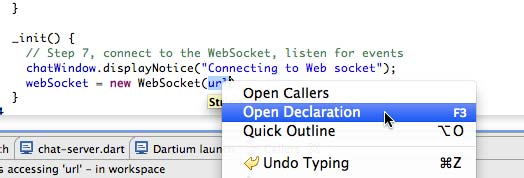
\includegraphics{step7/img_56.jpg}

urlはChatConnectionのインスタンス変数で、コンストラクタ内で設定されていることに注意してください。

\subsubsection{WebSocketイベントをハンドルする}

WebSocketオブジェクトは、open、close、error、messageの4つのイベントを返します。messageイベントは、WebSocketサーバから新しいメッセージを受信したことを通知します。メッセージの内容は、event.dataで取得することができます。

ヒント: WebSocketイベントのAPIドキュメントは http://api.dartlang.org/html/WebSocketEvents.html を参照してください。

ChatConnectionの\_initに、WebSocketイベントのハンドラを追加します。

\begin{verbatim}
// client/chat-client.dart
_init() {
  // Step 7. WebSocketサーバへ接続し、イベントを受信する。
  chatWindow.displayNotice("Connecting to Web socket");
  webSocket = new WebSocket(url);
  webSocket.on.open.add((e) {
    chatWindow.displayNotice('Connected');
  });
  webSocket.on.close.add((e) {
    chatWindow.displayNotice('web socket closed');
  });
  webSocket.on.error.add((e) {
    chatWindow.displayNotice("Error connecting to ws");
  });
  webSocket.on.message.add((e) {
    print('received message ${e.data}');
  });
}
\end{verbatim}

これでWebSocketイベントを利用する準備は完了したので、Step5で作成した\_receivedEncodedMessage()を利用しましょう。

\begin{verbatim}
// client/chat-client.dart
webSocket.on.message.add((e) {
  print('received message ${e.data}');
    _receivedEncodedMessage(e.data);
  });
\end{verbatim}

\subsubsection{WebSocketサーバへメッセージを送信する}

webSocketインスタンスが接続している状態では、WebSocketサーバに対してメッセージを送信することができます。ChatConnectionクラスの\_sendEncodedMessage()を探し、WebSocketサーバにエンコードされたメッセージを送信するコードを追加しましょう。webSocket変数がnullでは無く、接続が完了している場合のみメッセージを送信します。

\begin{verbatim}
// client/chat-client.dart
_sendEncodedMessage(String encodedMessage) {
  // Step 7. WebSocketサーバへメッセージを送信する。
  if (webSocket != null && webSocket.readyState == WebSocket.OPEN) {
    webSocket.send(encodedMessage);
  } else {
    print('WebSocket not connected, message $encodedMessage not sent');
  }
}
\end{verbatim}

\subsubsection{アプリを動かしてみよう}

サーバとクライアントを接続し、アプリを動かしてみましょう!

もしchat-server.dartを起動していないのなら、まず起動します。(起動方法はStep2を参照してください) 次に、client/chat-client.dartをDartiumのlaunchesから起動します。WebSocketサーバに接続成功すると、[system]: Connectedとチャットウインドウに表示されるでしょう。

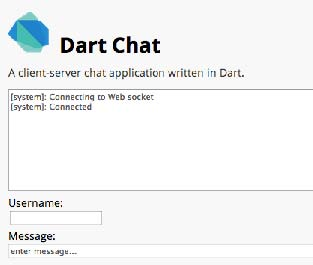
\includegraphics{step7/img_60.jpg}

Dart Editorのchat-server.dartの出力にnew ws conn messageと表示されていることをチェックし、クライアントがWebSocketサーバに接続したことを確認します。

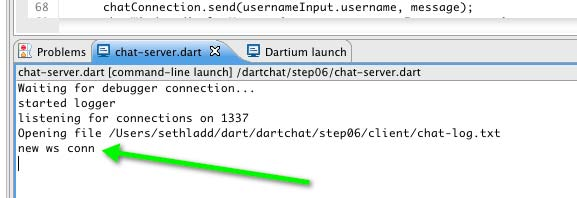
\includegraphics{step7/img_61.jpg}

サーバに接続できない場合は、chat-server.dartが起動しているか確認しましょう。また、Dartiumを終了し、再起動することも有効です。

いくつかメッセージを送受信してみましょう! DariumのURLをコピーし、Dartiumで新しいタブを開きます。そしてURLを貼り付けます。違うユーザ名を入力し、二つのウインドウの間でチャットをしてみましょう。

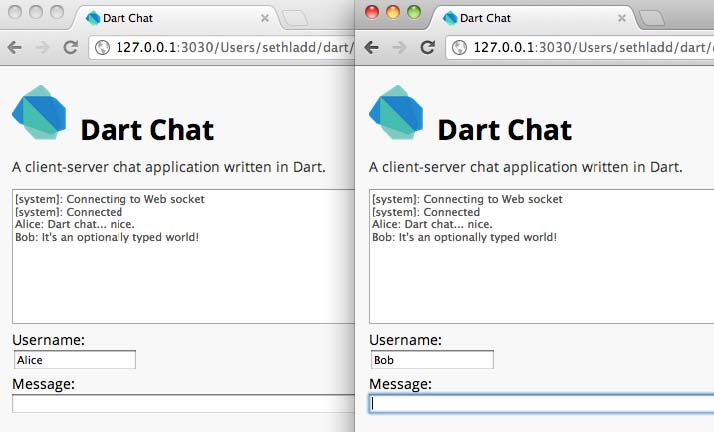
\includegraphics{step7/img_62.jpg}

\subsection{上級編}

接続失敗時に接続をリトライする処理を追加します。その際、リトライを試す間隔は徐々に増やします。

接続を試す前に数秒待つように\_init()を更新します。また、エラーが発生したかどうかを示すbooleanを追加します。

\begin{verbatim}
// client/chat-client.dart
_init([int retrySeconds = 2]) {
  // Step 6
  bool encounteredError = false;
\end{verbatim}

closeとerrorイベントハンドラーでは、遅延のあと再接続を試みます。closeとerrorハンドラの両方でencounteredError変数をtrueにし、リトライタイマーを一度だけスケジュールします。

\begin{verbatim}
// client/chat-client.dart
webSocket.on.close.add((e) {
  chatWindow.displayNotice('web socket closed, retrying in $retrySeconds seconds');
  if (!encounteredError) {
    window.setTimeout(() => _init(retrySeconds*2), 1000*retrySeconds);
  }
  encounteredError = true;
});
webSocket.on.error.add((e) {
  chatWindow.displayNotice("Error connecting to ws");
  if (!encounteredError) {
    window.setTimeout(() => _init(retrySeconds*2), 1000*retrySeconds);
  }
  encounteredError = true;
});
\end{verbatim}

setTimeout()メソッドは二つの引数を取ります。functionとそれをいつ呼び出すか(現在からのミリ秒)です。この場合はretrySeconds秒の後、\_init()メソッドを呼び出します。これはDartにおけるクロージャーの良い例です。setTimeout()メソッドに渡すインライン関数から、容易に\_init()メソッドとretrySeconds変数を参照することができます。

